 
\documentclass{article}
\usepackage[utf8]{inputenc}
\usepackage[italian]{babel}
\usepackage{graphicx}
\usepackage{cite}
\usepackage[hidelinks]{hyperref}
\usepackage{listings}
\usepackage{latexsym}
\usepackage{amsmath}
\usepackage{proof}
\usepackage{stmaryrd}
\usepackage{amssymb}
\usepackage{epstopdf}
\usepackage{pgf}
\usepackage{tikz}

\usetikzlibrary{positioning, arrows,calc,shapes,decorations.pathreplacing}

\usepackage[noend]{algpseudocode}
\usepackage[ruled,noline,linesnumbered]{algorithm2e}
\let\emptyset\varnothing

\graphicspath{ {./images/} }

%%Notation:

%%vectors
\renewcommand{\vec}[1]{\boldsymbol{#1}}
%%sets
\newcommand{\set}[1]{\mathcal{#1}}
%%matrixes
\newcommand{\mat}[1]{#1}
%%norm
\newcommand{\norm}[1]{\left\Vert #1 \right\Vert}
%%defeq
\newcommand{\defeq}{\triangleq}
%%
\newcommand{\net}[1]{\mathrm{#1}}
%% pair<x,y>
\newcommand{\pair}[2]{\langle#1,#2\rangle}
\usepackage{array}
\newcolumntype{C}[1]{>{\centering\arraybackslash}p{#1}}
\title{Lupus prospect}
\author{Giulio Galvan}

\begin{document}



\begin{table}[!h]
	\centering
	\begin{tabular}{C{1cm}  C{1cm}  C{1cm} | C{2cm} C{2cm} C{2cm} |  c c}
		upper span age & lower span age & min visits & AUC score (only features with variance among visits) & AUC score (all features but age) & AUC score (all features)& pos & neg\\\\
		0.8 & 0.8 & 1 & 0.58 & 0.60 & 0.63 & 38 & 143\\
		0.8 & 0.8 & 2 & 0.60 & 0.60 & 0.66 & 38 & 138\\
		0.8 & 0.8 & 3 & 0.58 & 0.67 & 0.71 & 38 & 124\\
		0.8 & 0.8 & 4 & 0.63 & 0.68 & 0.69 & 38 & 115\\
		0.8 & 0.8 & 5 & 0.71 & 0.73 & 0.74 & 38 & 94\\
		1.0 & 0.8 & 1 & 0.59 & 0.63 & 0.69 & 38 & 141\\
		1.0 & 0.8 & 2 & 0.56 & 0.62 & 0.68 & 38 & 133\\
		1.0 & 0.8 & 3 & 0.60 & 0.64 & 0.68 & 38 & 121\\
		1.0 & 0.8 & 4 & 0.53 & 0.71 & 0.69 & 38 & 108\\
		1.0 & 0.8 & 5 & 0.72 & 0.74 & 0.74 & 38 & 88\\
		2.0 & 0.8 & 1 & 0.59 & 0.69 & 0.72 & 38 & 99\\
		2.0 & 0.8 & 2 & 0.61 & 0.68 & 0.71 & 38 & 97\\
		2.0 & 0.8 & 3 & 0.72 & 0.71 & 0.73 & 38 & 90\\
		2.0 & 0.8 & 4 & 0.58 & 0.72 & 0.74 & 38 & 70\\
		2.0 & 0.8 & 5 & 0.70 & 0.72 & 0.69 & 38 & 48\\
		0.8 & 1.0 & 1 & 0.55 & 0.62 & 0.64 & 38 & 138\\
		0.8 & 1.0 & 2 & 0.54 & 0.62 & 0.69 & 38 & 133\\
		0.8 & 1.0 & 3 & 0.55 & 0.64 & 0.66 & 38 & 122\\
		0.8 & 1.0 & 4 & 0.56 & 0.68 & 0.67 & 38 & 114\\
		0.8 & 1.0 & 5 & 0.69 & 0.73 & 0.69 & 38 & 93\\
		1.0 & 1.0 & 1 & 0.53 & 0.61 & 0.67 & 38 & 134\\
		1.0 & 1.0 & 2 & 0.54 & 0.62 & 0.64 & 38 & 127\\
		1.0 & 1.0 & 3 & 0.53 & 0.65 & 0.73 & 38 & 118\\
		1.0 & 1.0 & 4 & 0.57 & 0.69 & 0.73 & 38 & 107\\
		1.0 & 1.0 & 5 & 0.68 & 0.72 & 0.70 & 38 & 87\\
		2.0 & 1.0 & 1 & 0.60 & 0.67 & 0.69 & 38 & 89\\
		2.0 & 1.0 & 2 & 0.59 & 0.69 & 0.72 & 38 & 87\\
		2.0 & 1.0 & 3 & 0.60 & 0.67 & 0.73 & 38 & 83\\
		2.0 & 1.0 & 4 & 0.64 & 0.72 & 0.74 & 38 & 67\\
		2.0 & 1.0 & 5 & 0.69 & 0.72 & 0.69 & 38 & 48\\
		0.8 & 2.0 & 1 & 0.57 & 0.65 & 0.63 & 38 & 97\\
		0.8 & 2.0 & 2 & 0.62 & 0.66 & 0.67 & 38 & 95\\
		0.8 & 2.0 & 3 & 0.57 & 0.69 & 0.70 & 38 & 92\\
		0.8 & 2.0 & 4 & 0.57 & 0.70 & 0.68 & 38 & 91\\
		0.8 & 2.0 & 5 & 0.60 & 0.69 & 0.70 & 38 & 83\\
		1.0 & 2.0 & 1 & 0.59 & 0.69 & 0.64 & 38 & 88\\
		1.0 & 2.0 & 2 & 0.53 & 0.69 & 0.64 & 38 & 86\\
		1.0 & 2.0 & 3 & 0.60 & 0.71 & 0.66 & 38 & 85\\
		1.0 & 2.0 & 4 & 0.50 & 0.67 & 0.62 & 38 & 84\\
		1.0 & 2.0 & 5 & 0.67 & 0.69 & 0.67 & 38 & 74\\
		2.0 & 2.0 & 1 & 0.66 & 0.70 & 0.64 & 38 & 45\\
		2.0 & 2.0 & 2 & 0.63 & 0.67 & 0.68 & 38 & 44\\
		2.0 & 2.0 & 3 & 0.63 & 0.70 & 0.68 & 38 & 43\\
		2.0 & 2.0 & 4 & 0.56 & 0.70 & 0.70 & 38 & 41\\
		2.0 & 2.0 & 5 & 0.59 & 0.69 & 0.66 & 38 & 35\\
	\end{tabular}
	\caption{AUC ROC score for different training sets. Best score in bold.}
	\label{table:exp_res}
\end{table}


%\begin{figure}[!h]
%	\centering
%	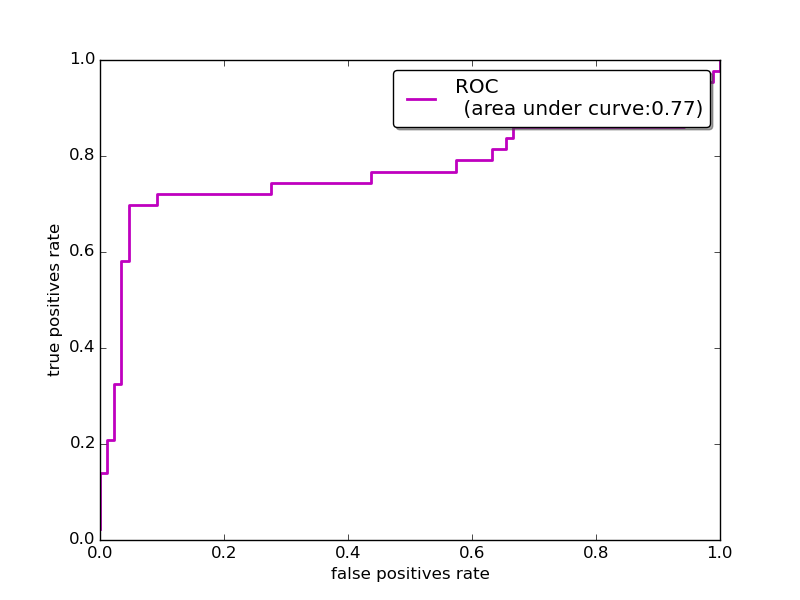
\includegraphics[width= 0.8\textwidth]{roc.png}
%	\caption{roc curve for the best model}
%	\label{fig:roc_best}
%\end{figure}
%
%\begin{figure}[!h]
%	\centering
%	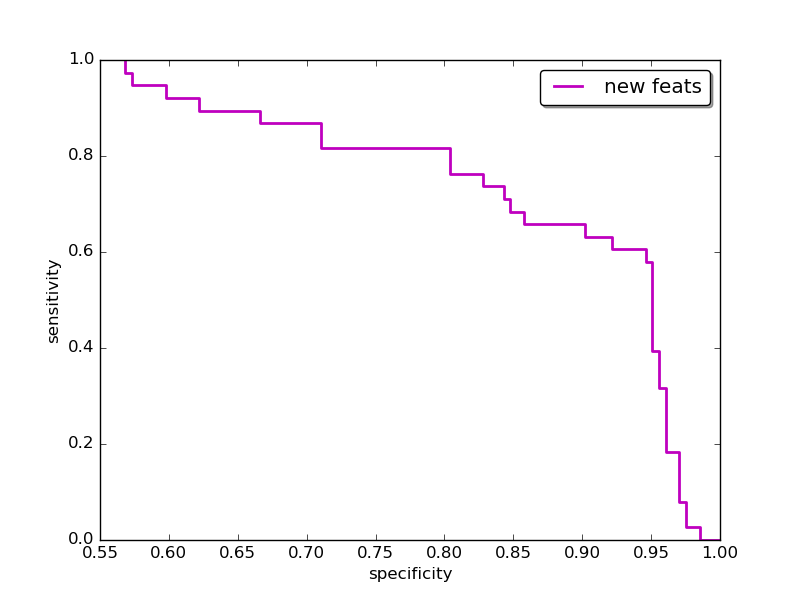
\includegraphics[width= 0.8\textwidth]{sensibility_specificity.png}
%	\caption{sensibility-specificity curve for the best model}
%	\label{fig:sensibility_specificity_best}
%\end{figure}
%
%\begin{figure}[!h]
%	\centering
%	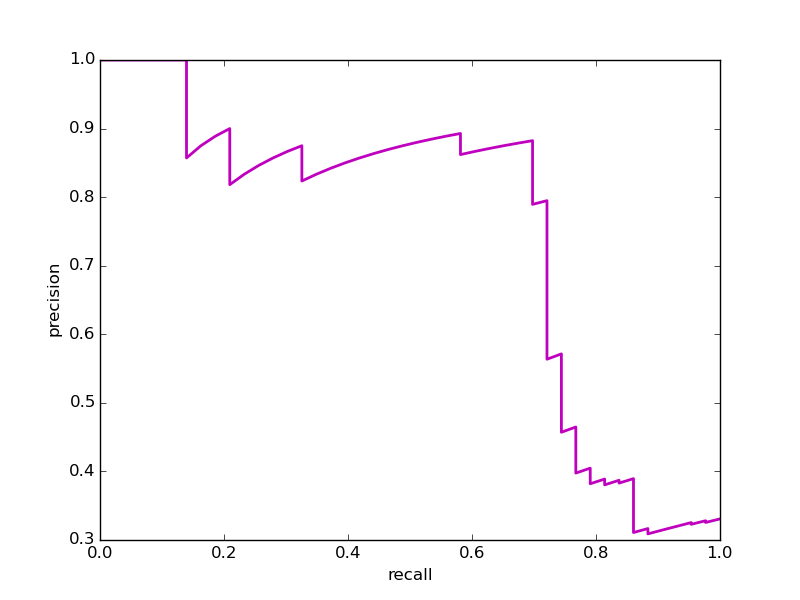
\includegraphics[width= 0.8\textwidth]{precision_recall.png}
%	\caption{precision-recall curve for the best model}
%	\label{fig:precision_recall_best}
%\end{figure}


\end{document}      


